\begin{figure}[!p]
    \centering
    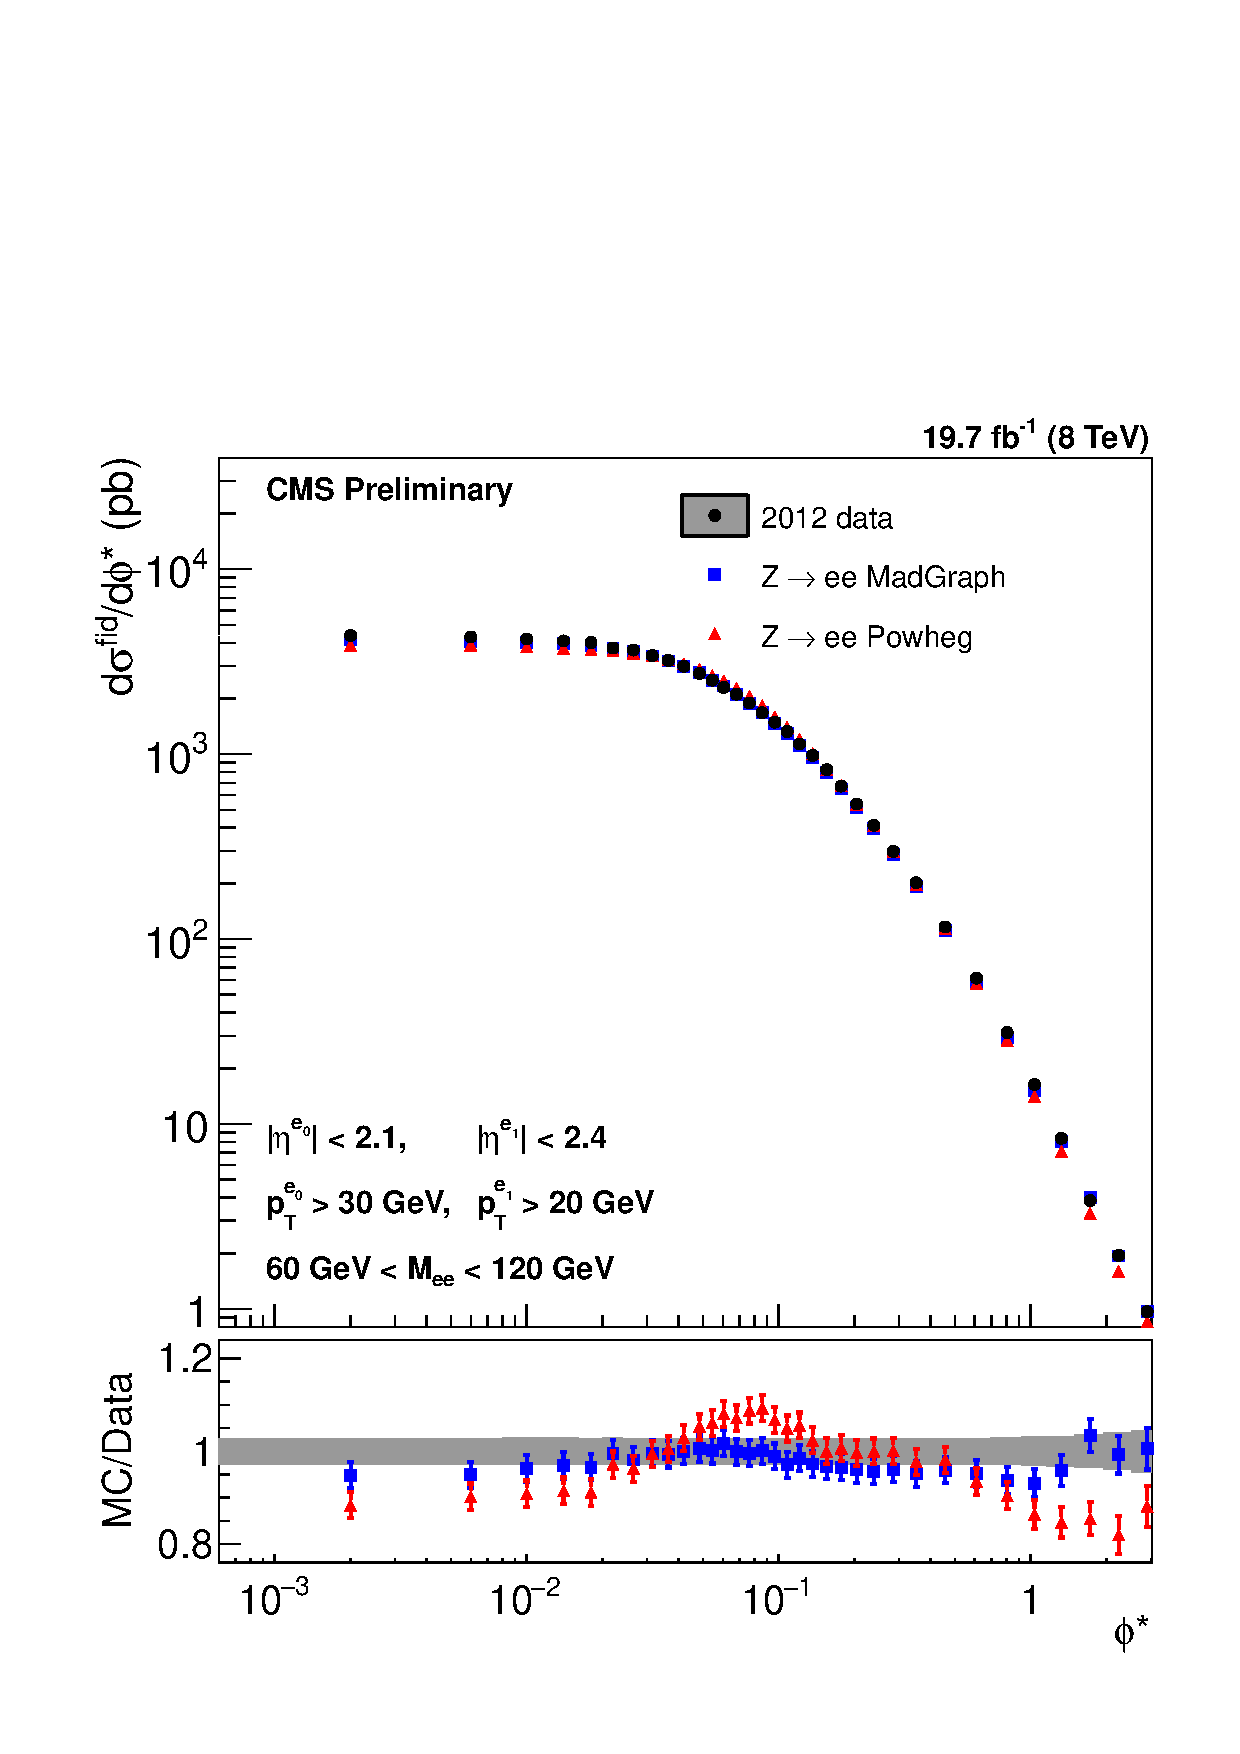
\includegraphics[width=\textwidth]{figures/ZShape_elec_PH_Abs_Dressed.pdf}
    \caption[
        The absolute differential cross section with respects to \phistar for
        \Ztoee events in our fiducial region from data unfolded with \POWHEG,
        and the same distributions in \MADGRAPH and \POWHEG.
    ]{
        The absolute differential cross section with respects to \phistar for
        \Ztoee events in our fiducial region from data unfolded with \POWHEG,
        and the same distributions in \MADGRAPH and \POWHEG. A close up of the
        lower plot is shown in \cref{fig:results_ratio_abs_powheg}.
    }
    \label{fig:results_abs_powheg}
\end{figure}

\begin{figure}[!p]
    \centering
    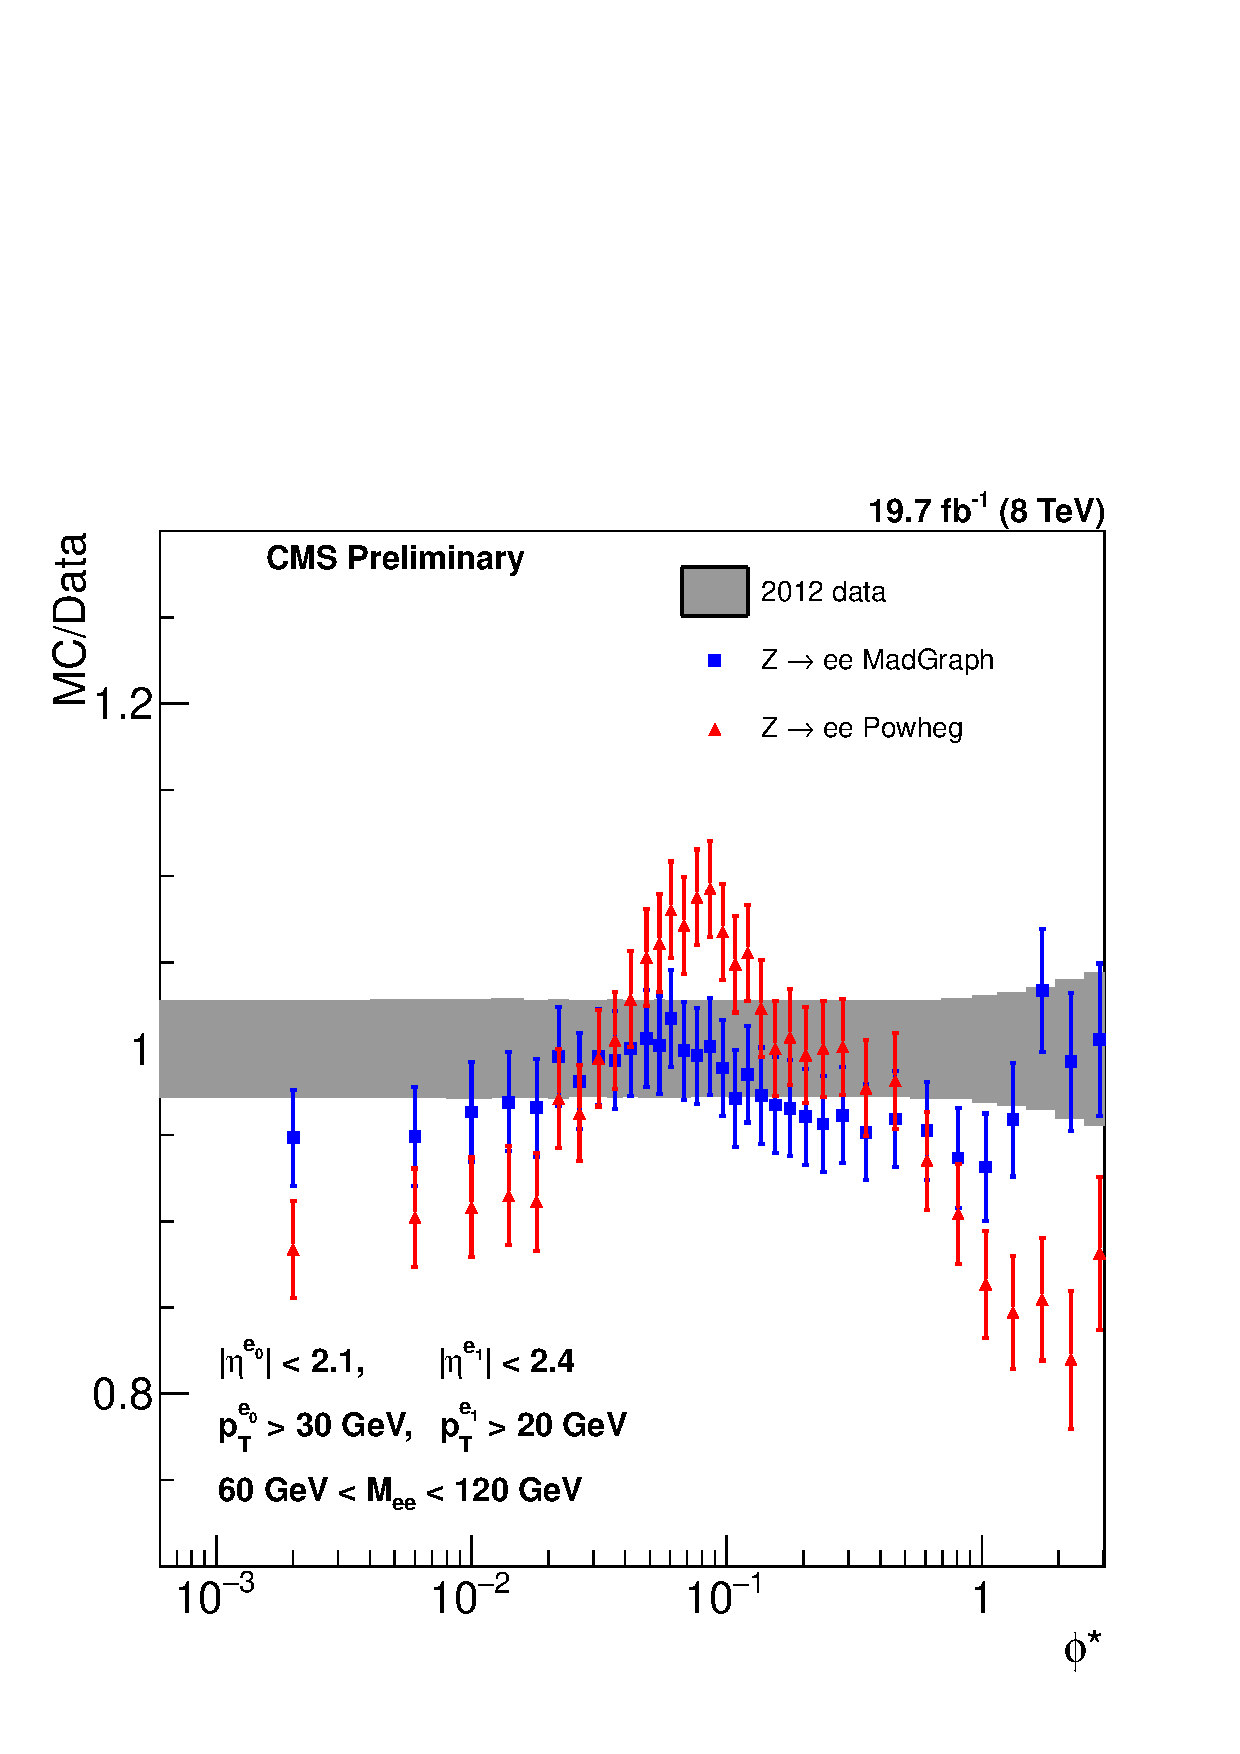
\includegraphics[width=\textwidth]{figures/ZShape_Ratioelec_PH_Abs_Dressed.pdf}
    \caption[
        Close up of the ratio plot from \cref{fig:results_abs_powheg} for
        the absolute cross section measurement unfolded with \POWHEG.
    ]{
        Close up of the ratio plot from \cref{fig:results_abs_powheg} for
        the absolute cross section measurement unfolded with \POWHEG. The error
        band indicates the uncertainty in the data, while the square points
        show the ratio of \MADGRAPH over data, and the triangle points show the
        ratio of \POWHEG over data.
    }
    \label{fig:results_ratio_abs_powheg}
\end{figure}
